\documentclass[10pt]{beamer}

\usepackage[utf8]{inputenc}
% Remove russian in English presentation
\usepackage[english,russian]{babel}

\usetheme[
  sectionpage=simple,
  numbering=fraction
]{metropolis}
\usepackage{appendixnumberbeamer}

\usepackage{booktabs}
\usepackage[scale=2]{ccicons}

\usepackage{pgfplots}
\usepgfplotslibrary{dateplot}

\usepackage{xspace}
\usepackage{svg}
\newcommand{\themename}{\textbf{\textsc{metropolis}}\xspace}

\usepackage{todonotes}
\usepackage{ifthen}%
\providecommand\enabletodos{true}%
\ifthenelse{ \equal{\enabletodos}{true} }{%
  \presetkeys{todonotes}{inline}{}%
}{%
  \presetkeys{todonotes}{disable}{}%
}%

\setbeamertemplate{caption}{\raggedright\insertcaption\par}

\AtBeginSection[]{}

\setbeamertemplate{section in toc}{%
  \alert{$\bullet$}~\inserttocsection}
\setbeamercolor{subsection in toc}{bg=white,fg=structure}
\setbeamertemplate{subsection in toc}{%
  \hspace{1.2em}{\alert{\rule[0.3ex]{3pt}{3pt}}~\inserttocsubsection\par}}

\usepackage{hyperref}
\hypersetup{unicode=true}

\setbeamertemplate{caption}[numbered]
\setbeamertemplate{table}[numbered]

\usepackage{adjustbox}
\protected\def\psverb#1{\def\innerpsverb##1#1{\texttt{##1}}\innerpsverb}
\usepackage{listings}

\usepackage{makecell}
\usepackage{changepage}

\title{Автоматическая генерация сигнатур сетевых протоколов}
%\subtitle{Подназвание доклада}
\date{18 апреля 2024 г.}
\author{{Дурнов Алексей Николаевич}\\
{Научный руководитель: к. ф.-м. н. Гетьман А. И.}
}

% Russian
\institute{МФТИ, кафедра системного программирования, ИСП РАН}
\titlegraphic{\hfill
\includegraphics[height=0.5cm]{logo_isp_ru.png}}
% English
% \institute{ISP RAS}
% \titlegraphic{\hfill
\includegraphics[height=0.5cm]{logo_isp_en.png}}

\definecolor{Blue}{HTML}{29619b}
\setbeamercolor{frametitle}{bg=Blue}
\setbeamercolor{palette primary}{bg=Blue}

\begin{document}

\maketitle

\begin{frame}{Введение}
    \begin{itemize}
      \item Методы классификации сетевого трафика:
        \begin{enumerate}
            \item основанные на идентификации по номеру порта сервера
            \item основанные на DPI подходе
            \begin{itemize}
                \item \alert{сигнатурный}
            \end{itemize}
            \item основанные на статистических характеристиках
        \end{enumerate}
        \item Свойства сигнатур для сетевых протоколов и приложений:
        \begin{enumerate}
            \item короткие общие подстроки
            \item несколько потоков с разным набором подстрок
            \item необходимость частого обновления
        \end{enumerate}
    \end{itemize}
\end{frame}

\begin{frame}{Цель}
    Целью данной работы является разработка и реализация метода автоматической
    генерации сигнатур полезной нагрузки сетевого трафика для классификации этого трафика
    в соответствии с использующимся протоколом.
\end{frame}

\begin{frame}{Задачи}
    \begin{itemize}
        \item Провести исследование литературы по соответствующей теме.
        \item Собрать набор сетевых трасс для последующего тестирования.
        \item Выбрать формат сигнатуры сетевых протоколов.
        \item Разработать алгоритм генерации сигнатур.
        \begin{enumerate}
            \item Выбрать методы для автоматической генерации сигнатур.
            \item Рассмотреть ограничения данных методов.
        \end{enumerate}
        \item Разработать классификатор сетевого трафика для проверки сгенерированных сигнатур.
        \begin{enumerate}
            \item Реализовать сопоставление сигнатур.
            \item Выбрать метрики, по котором можно оценить качество классификации сигнатур.
        \end{enumerate}
        \item Встроить генератор сигнатур и классификатор как модули в систему анализа высокоскоростного сетевого трафика, разрабатываемую в ИСП РАН.
    \end{itemize}
\end{frame}

\begin{frame}{Формат сигнатур}
    \begin{itemize}
        \item Сигнатура - набор последовательностей подстрок (байт).
        \item Полезная нагрузка соотвествует
        сигнатуре, если она содержит какую-то последовательность подстрок из этого набора.
        \item Иерархия сигнатур:
        \begin{enumerate}
            \item сигнатура содержимого
            \item сигнатура пакета
            \item сигнатура потока
        \end{enumerate}
    \end{itemize}
\end{frame}

\begin{frame}{Формат сигнатур: иерархия}
    \begin{figure}
        \begin{adjustwidth}{-2em}{-2em}
            \centering
            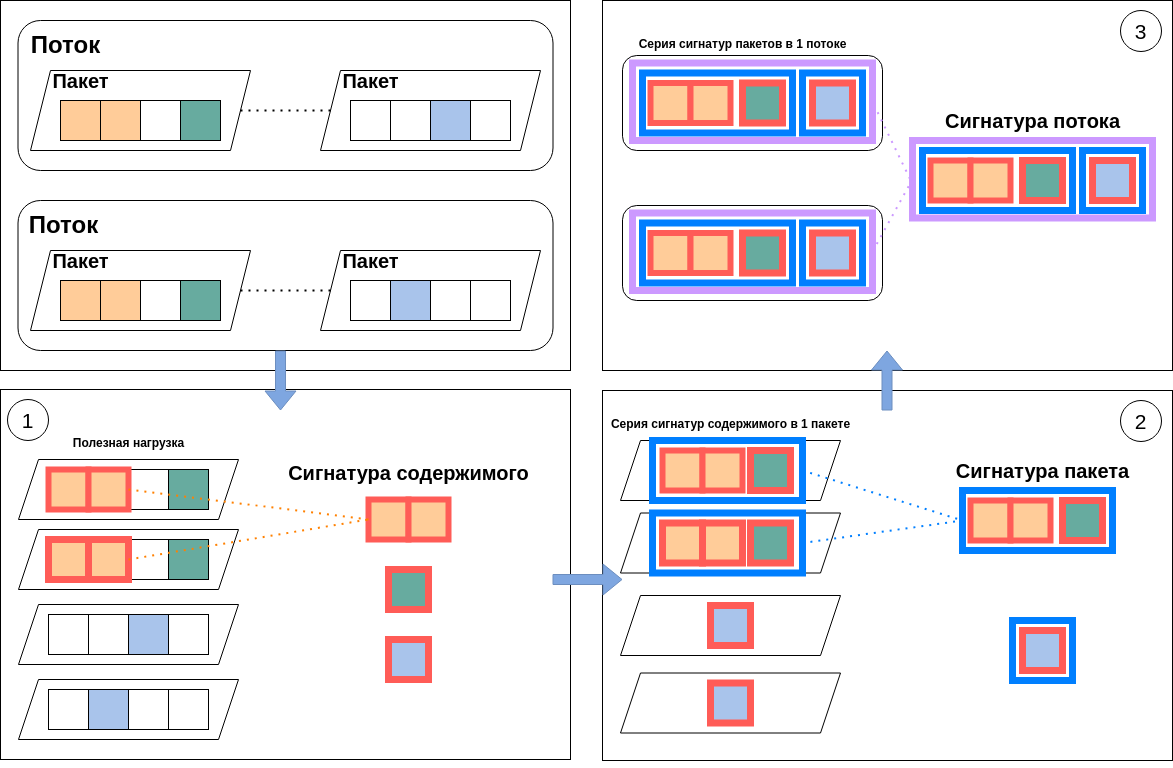
\includegraphics[width=25em]{../images/signature_structure.png}
        \end{adjustwidth}
    \end{figure}

\end{frame}

\begin{frame}{Методы автоматической генерации сигнатур}

    \begin{itemize}
        \item \alert{LASER} (Application Signature ExtRaction)
        \begin{itemize}
            \item \alert{LCS} (Long Common Subsequence)
            \item cигнатура пакета
            \item[+] наиболее подходящий для модификаций
            \item[---] неустойчив к шумам
            \item[---] не утилизирует все потоки
        \end{itemize}
        \item AutoSig
        \begin{itemize}
            \item cигнатура потока
            \item[+] набор последовательностей подстрок
            \item[+] учитывает частотное распределение подстрок
            \item[---] избыточное дерево подстрок
            \item[---] долгая сходимость алгоритма
        \end{itemize}
        \item SigBox
        \begin{itemize}
            \item cигнатура потока
            \item[+] поддерживает иерархию
            \item[---] долгая сходимость алгоритма
        \end{itemize}
    \end{itemize}

\end{frame}

\begin{frame}{Схема генерации сигнатуры}
    \begin{figure}
        \begin{adjustwidth}{-2em}{-2em}
            \centering
            \includesvg[width=27em]{../images/scheme_auto_signature_generation}
        \end{adjustwidth}
    \end{figure}
\end{frame}

\begin{frame}{Схема классификации трафика}
    \begin{figure}
        \begin{adjustwidth}{-2em}{-2em}
            \centering
            \includesvg[width=27em]{../images/scheme_auto_signature_classifier}
        \end{adjustwidth}
    \end{figure}
\end{frame}

\begin{frame}[shrink=5]{Данные для генерации сигнатур}
    \begin{table}[]
        \resizebox{12cm}{!}{
            \begin{tabular}{|c|c|c|c|c|c|c|}
                \hline
                Протокол   & \begin{tabular}[c]{@{}c@{}}Размер, \\ МБ\end{tabular} & \begin{tabular}[c]{@{}c@{}}Количество \\ пакетов\end{tabular} & \begin{tabular}[c]{@{}c@{}}Количество \\ потоков\end{tabular} &  \begin{tabular}[c]{@{}c@{}}Avg \\ bytes/pkt \end{tabular} &  \begin{tabular}[c]{@{}c@{}}Avg \\ pkts/stream \end{tabular} & \begin{tabular}[c]{@{}c@{}} Количеcтво \\ потоков: \\ $\geq$ 5 pkts \end{tabular} \\ \hline
                bittorrent & 272,4      & 240159             & 708                & 1134                             & 339                                 & 214                                          \\ \hline
                dns        & 130,7      & 1283082            & 204150             & 102                              & 6                                   & 11027                                        \\ \hline
                ftp        & 0,86       & 16959              & 735                & 51                               & 23                                  & 725                                          \\ \hline
                http       & 1811,5     & 799062             & 13710              & 2268                             & 58                                  & 1500                                         \\ \hline
                imap       & 22,0       & 27702              & 66                 & 793                              & 419                                 & 65                                           \\ \hline
                pop        & 0,06       & 919                & 59                 & 64                               & 16                                  & 40                                           \\ \hline
                smtp       & 13,5       & 59121              & 1120               & 229                              & 53                                  & 799                                          \\ \hline
            \end{tabular}}
    \end{table}
\end{frame}

\begin{frame}[shrink=5]{Данные для классификации}


    \begin{table}[]
        \resizebox{12cm}{!}{
            \begin{tabular}{|c|c|c|c|c|c|}
                \hline
                Протокол   & \begin{tabular}[c]{@{}c@{}}Размер, \\ МБ\end{tabular} & \begin{tabular}[c]{@{}c@{}}Количество \\ пакетов\end{tabular} & \begin{tabular}[c]{@{}c@{}}Количество \\ потоков\end{tabular} &  \begin{tabular}[c]{@{}c@{}}Avg \\ bytes/pkt \end{tabular} &  \begin{tabular}[c]{@{}c@{}}Avg \\ pkts/stream \end{tabular}\\ \hline
                bittorrent & 1,26       & 9409               & 876                & 133                              & 11                                  \\ \hline
                dns        & 53,3       & 664809             & 27800              & 80                               & 24                                  \\ \hline
                ftp        & 0,19       & 4000               & 294                & 48                               & 14                                  \\ \hline
                http       & 1494       & 406030             & 4607               & 3681                             & 88                                  \\ \hline
                imap       & 3,38       & 10587              & 143                & 320                              & 74                                  \\ \hline
                other      & 1119       & 1235122            & 18846              & 906                              & 66                                  \\ \hline
                pop        & 0,02       & 344                & 21                 & 58                               & 16                                  \\ \hline
                smtp       & 5,8        & 34428              & 1018               & 170                              & 34                                  \\ \hline
            \end{tabular}}
        \end{table}
\end{frame}

\begin{frame}{Генерация сигнатур: алгоритм LASER}
    \begin{table}[]
        \begin{tabular}{|c|c|c|}
        \hline
        Протокол & Количество сигнатур & \begin{tabular}[c]{@{}c@{}}Среднее количество \\ потоков на 1 сигнатуру\end{tabular} \\ \hline
        bittorent & 51                  & 4,1                                       \\ \hline
        dns       & 682                 & 16,1                                      \\ \hline
        ftp       & 9                   & 80,5                                     \\ \hline
        http      & 145                 & 10,3                                      \\ \hline
        imap      & 10                  & 6,5                                       \\ \hline
        pop       & 2                   & 20,0                                      \\ \hline
        smtp      & 167                 & 4,8                                       \\ \hline
        \end{tabular}
        \end{table}
\end{frame}

\begin{frame}{Результаты работы алгоритма LASER}
    \begin{figure}
        \begin{adjustwidth}{-2em}{-2em}
            \centering
            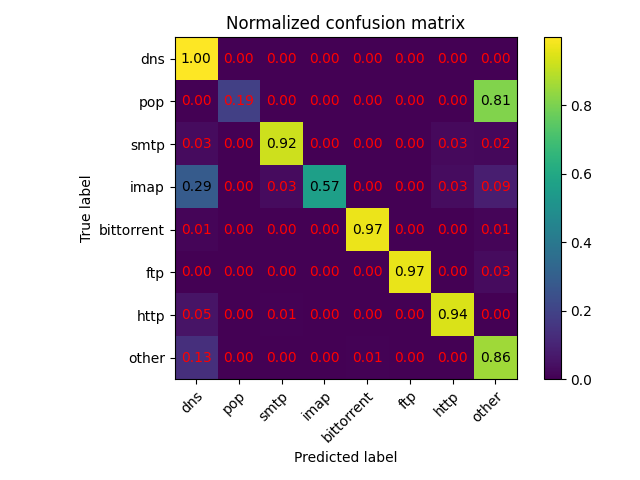
\includegraphics[width=27em]{results/laser_no_filtered/Normalized_confusion_matrix.png}
        \end{adjustwidth}
    \end{figure}
\end{frame}

\begin{frame}{Результаты работы алгоритма LASER}
    \begin{table}[]
        \begin{tabular}{|c|c|c|c|c|}
        \hline
        protocol     & precision & recall & f1-score & support \\ \hline
        dns          & 0.93      & 1.00   & 0.97     & 27801   \\ \hline
        pop          & 0.80      & 0.19   & 0.31     & 21      \\ \hline
        smtp         & 0.94      & 0.92   & 0.93     & 1076    \\ \hline
        imap         & 1.00      & 0.57   & 0.72     & 175     \\ \hline
        bittorrent   & 0.92      & 0.97   & 0.95     & 886     \\ \hline
        ftp          & 0.99      & 0.97   & 0.98     & 295     \\ \hline
        http         & 0.99      & 0.94   & 0.96     & 4888    \\ \hline
        other        & 0.99      & 0.86   & 0.92     & 12094   \\ \hline
                     &           &        &          &         \\ \hline
        accuracy     &           &        & 0.95     & 47236   \\ \hline
        macro avg    & 0.95      & 0.80   & 0.84     & 47236   \\ \hline
        weighted avg & 0.95      & 0.95   & 0.95     & 47236   \\ \hline
        \end{tabular}
        \end{table}
\end{frame}

\begin{frame}{Постобработка: \\ удаление дубликатов и простых надмножеств}

    \begin{table}[]
        \resizebox{6cm}{!}{
        \begin{tabular}{|c|cc|cc|}
        \hline
        Протокол & \multicolumn{2}{c|}{\begin{tabular}[c]{@{}c@{}}Количество\\ сигнатур\end{tabular}} & \multicolumn{2}{c|}{Избыточность} \\ \cline{2-5}
                   & \multicolumn{1}{c|}{Было} & Стало & \multicolumn{1}{c|}{Было} & Стало \\ \hline
        bittorrent & \multicolumn{1}{c|}{51}   & 7     & \multicolumn{1}{c|}{0.53} & 0.53  \\ \hline
        dns        & \multicolumn{1}{c|}{682}  & 64    & \multicolumn{1}{c|}{0.99} & 0.99  \\ \hline
        ftp        & \multicolumn{1}{c|}{9}    & 8     & \multicolumn{1}{c|}{0.98} & 0.98  \\ \hline
        http       & \multicolumn{1}{c|}{145}  & 47    & \multicolumn{1}{c|}{1.00} & 1.00  \\ \hline
        imap       & \multicolumn{1}{c|}{10}   & 4     & \multicolumn{1}{c|}{1.00} & 0.79  \\ \hline
        pop        & \multicolumn{1}{c|}{2}    & 1     & \multicolumn{1}{c|}{1.00} & 0.00  \\ \hline
        smtp       & \multicolumn{1}{c|}{167}  & 26    & \multicolumn{1}{c|}{0.99} & 0.99  \\ \hline
        \end{tabular}}
    \end{table}

    \begin{itemize}
        \item Избыточность - отношение числа потоков, идентифицированных двумя и более сигнатурами к общему числу потоков, идентифицированных набором сигнатур.
        \item Результаты классификации никак не поменялись, при этом сильно упало количество сигнатур.
        \item Слегка уменьшилась избыточность.
    \end{itemize}
\end{frame}

\begin{frame}{Схема генерации сигнатуры со сборкой TCP-сессий}
    \begin{figure}
        \begin{adjustwidth}{-2em}{-2em}
            \centering
            \includesvg[width=27em]{../images/scheme_auto_signature_generation_v2}
        \end{adjustwidth}
    \end{figure}
\end{frame}

\begin{frame}{Схема классификации трафика со сборкой TCP-сессий}
    \begin{figure}
        \begin{adjustwidth}{-2em}{-2em}
            \centering
            \includesvg[width=27em]{../images/scheme_auto_signature_classifier_v2}
        \end{adjustwidth}
    \end{figure}
\end{frame}

\begin{frame}{Результаты работы алгоритма LASER: \\ со сборкой последовательных пакетов TCP-сессии}
    \begin{figure}
        \begin{adjustwidth}{-2em}{-2em}
            \centering
            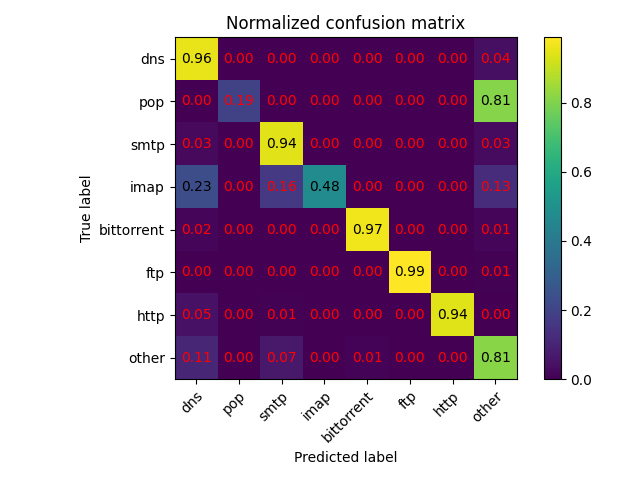
\includegraphics[width=27em]{results/laser_reasm/Normalized_confusion_matrix.png}
        \end{adjustwidth}
    \end{figure}
\end{frame}

\begin{frame}{Результаты работы алгоритма LASER: \\ со сборкой последовательных пакетов TCP-сессии}
    \begin{table}[]
        \begin{tabular}{|c|c|c|c|c|}
        \hline
        protocol     & precision & recall & f1-score & support \\ \hline
        dns          & 0.92      & 0.96   & 0.94     & 10565   \\ \hline
        pop          & 0.67      & 0.19   & 0.30     &    21   \\ \hline
        smtp         & 0.78      & 0.94   & 0.85     &  1464   \\ \hline
        imap         & 0.91      & 0.48   & 0.62     &   189   \\ \hline
        bittorrent   & 0.95      & 0.97   & 0.96     &   853   \\ \hline
        ftp          & 0.99      & 0.99   & 0.99     &   288   \\ \hline
        http         & 1.00      & 0.94   & 0.97     &  4890   \\ \hline
        other        & 0.88      & 0.81   & 0.85     &  4804   \\ \hline
                     &           &        &          &         \\ \hline
        accuracy     &           &        & 0.92     & 23074   \\ \hline
        macro avg    & 0.89      & 0.79   & 0.81     & 23074   \\ \hline
        weighted avg & 0.92      & 0.92   & 0.92     & 23074   \\ \hline

        \end{tabular}
    \end{table}
\end{frame}

\begin{frame}{Результаты}
    \begin{itemize}
        \item При частичной сборке TCP-сессии c использованием LASER, полученные результаты получились немного хуже.
        \item При полной сборке TCP-сессии с использованием LCS, результаты сильно зависят от параметров алгоритма и постобработки. Параметры необходимо подбирать для каждого протокола вручную.
        \item Могут генерироваться неспецифичные сигнатуры.
    \end{itemize}
\end{frame}

\begin{frame}{Заключение}
    \begin{itemize}
        \item Проведено исследование литературы по соответствующей теме.
        \item Собран набор сетевых трасс для генерации и классификации.
        \item Выбран формат сигнатуры сетевых протоколов.
        \item Рассмотрены ограничения выбранных методов и реализован один из них.
        \item Разработан классификатор сетевого трафика для проверки сгенерированных сигнатур.
        \item Рассмотрено влияние сборки TCP-сессии и постобработки на результат классификации
        \item Встроены генератор сигнатур и классификатор как модули в систему анализа высокоскоростного сетевого трафика, разрабатываемую в ИСП РАН.
    \end{itemize}
\end{frame}

\begin{frame}{Будущие исследования}

    \begin{itemize}
        \item Реализация и сравнение других методов генерации сигнатур: AutoSig и SigBox.
        \item Реализация модуля уточнения положения сигнатуры и его влияние на точность.
        \item Рассмотрение возможности применения машинного обучения (метода SVM) для выбора набора сигнатур при постобработке результатов.
    \end{itemize}
\end{frame}

\appendix

\begin{frame}[standout] \vfill Спасибо за внимание \vfill \end{frame}

\end{document}
